\section{서론}

GPT-3 \citep{Brown2020GPT3}, GPT-4 \citep{OpenAI2023GPT4}, Gemini~\citep{team2023gemini}, DeepSeek-R1~\citep{guo2025deepseek} 같은 대규모 언어 모델(Large Language Models, LLMs)은 이제 인간과 유사한 언어 이해와 생성 능력을 보이며, 환경, 도구, 다른 에이전트와 상호작용하는 자율 에이전트로 활용될 수 있다 \citep{Wang2023CommunicativeAgents, Park2023GenerativeAgents, OpenAI2023FunctionCalling}. 단일 에이전트 시스템은 인상적인 역량을 입증했지만, 고립적으로 작동할 경우 과제 실행 효율이 제한될 수 있고 복잡하며 사회적으로 동적인 시나리오를 시뮬레이션하기에는 부족하다. 반대로 다중 에이전트(multi-agent) 구성 \citep{Li2023ChatDev, Wang2023Roleplaying, unleashing2024}은 여러 LLM 기반 에이전트가 협업하고, 조정하며, 공동으로 계획하도록 하여 이러한 문제를 다룬다. 이 패러다임은 과제 실행 효율을 높일 뿐 아니라 사회적 상호작용과 동역학을 현실적으로 시뮬레이션할 수 있게 하며, 전략적 의사결정, 게임 \citep{Silver2017Mastering}, 소프트웨어 개발 \citep{Wang2023CommunicativeAgents} 같은 영역의 성능을 향상시킨다.


% One particularly promising area is the development of LLM-based multi-agent systems, where multiple agents collaborate to tackle tasks that are beyond the capabilities of a single agent \citep{Li2023ChatDev, Wang2023Roleplaying}. These systems open up new possibilities for solving complex problems that require coordination, planning, and collective intelligence. For example, multi-agent collaboration has been shown to enhance performance in strategic games \citep{Silver2017Mastering}, cooperative decision-making \citep{Dafoe2020Open}, and collaborative software development \citep{Wang2023CommunicativeAgents}.

\begin{figure}[htbp]
    \centering
    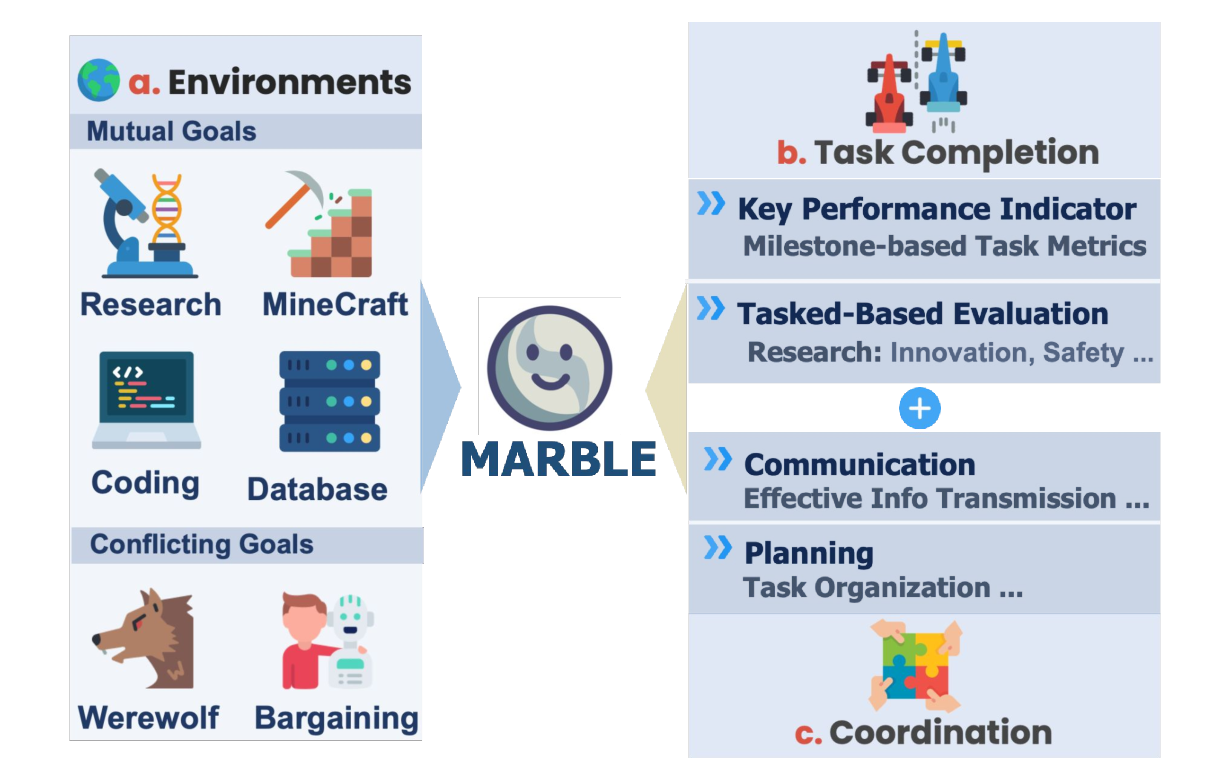
\includegraphics[width=\linewidth]{graphs/Introduction.pdf}
    \caption{\textbf{MultiAgentBench 평가 과정 개요}: 다양한 상호작용 환경에서의 다중 에이전트 시스템 조정을 보여 주며, 과제 성능과 조정에 초점을 둔다.}
    \label{fig:overview}
\end{figure}

%\cheng{Illustration still seems vague here, is it possible to add 1-2 sentences in the figure to explain the scenario or clearly indicates what the metrics measure? (given this figure tasks s much spaces?)}

% However, existing benchmarks and evaluations primarily emphasize single-agent interactions or do not fully capture the dynamics of multi-agent coordination. Approaches like MMLU \citep{Hendrycks2020Measuring} and HumanEval \citep{Chen2021Evaluating} assess language understanding or code generation in isolation. Agent-oriented frameworks such as GAIA \citep{Huang2023LanguageAgents} and AgentBench \citep{Lu2023AgentBench} focus on single-agent performance, while others \citep{Sun2023VisualAgentBench} center on narrow domains. Similarly, prior text-based games \citep{Urbanek2019Learning, Cote2019TextWorld, Hausknecht2020Interactive, Ammanabrolu2020Graph} or multi-modal simulators \citep{Kuttler2020NLE, Fan2022Minedojo, Shi2017WorldOfBits, Toyama2021WebArena, Shen2021iGibson, Srivastava2022Behavior} lack a comprehensive setting tailored to LLM-based multi-agent collaboration.
% \kunlun{Mention Why multiagent, 1.scenarios need multi-persona for simulation only multiagent work 2. benefits comparing to single agents: citing paper like scaling llm , the number increase the performance on coding task, benefits in the efficiency and expand the }

% \kunlun{Specify why original dataset would not elicit the cooperation easily}
% \kunlun{Previous constraints}

% Despite the growing interest, evaluating the effectiveness of LLM-based multi-agent systems remains a significant challenge. Current benchmarks predominantly focus on single-agent settings or evaluate task completion without accounting for multi-agent dynamics. Benchmarks like MMLU \citep{Hendrycks2020Measuring} and HumanEval \citep{Chen2021Evaluating} assess language understanding and code generation in isolation. Frameworks such as GAIA \citep{Huang2023LanguageAgents} and AgentBench \citep{Lu2023AgentBench} focus on single-agent interactions within environments that do not inherently require multi-agent coordination. Other works, like Visual Agent Bench \citep{Sun2023VisualAgentBench}, evaluate agent performance in specific domains but lack a comprehensive assessment of multi-agent collaboration.

% Historically, text-based game environments have been employed for language agent evaluation \citep{Urbanek2019Learning, Cote2019TextWorld, Hausknecht2020Interactive, Ammanabrolu2020Graph}. However, these environments often suffer from limitations such as closed, discrete action spaces and a narrow focus on commonsense grounding. Recent attempts on embodied agents have employed complex multi-modal simulators based on games \citep{Kuttler2020NLE, Fan2022Minedojo}, graphical user interfaces (GUIs) \citep{Shi2017WorldOfBits, Toyama2021WebArena}, and indoor scenes \citep{Shen2021iGibson, Srivastava2022Behavior}. Despite their complexity, these simulators do not accurately reflect the practical use cases of LLMs, and their multi-modal nature creates hurdles for the evaluation of existing text-only LLMs. Furthermore, most current benchmarks focus on single environments and fail to provide a comprehensive overview of LLMs across diverse application scenarios.
% \cheng{logic could be more coherent if written like this: what ability previous benchmarks emphasize? -> What are the unique traits that multi-agent benchmark demands? -> all previous ones fail to capture these traits -> this motivates our design}
% Despite these advances, current evaluation paradigms remain inadequate for multi-agent scenarios. Single-agent benchmarks like \kunlun{agentbench, GAIA}, MMLU \citep{Hendrycks2020Measuring} and HumanEval \citep{Chen2021Evaluating} fail to capture coordination dynamics, while domain-specific frameworks \citep{Sun2023VisualAgentBench} lack cross-task generalizability. Text-based games \citep{Ammanabrolu2020Graph} and multi-modal simulators \citep{Srivastava2022Behavior} either impose restrictive action spaces or require non-textual interfaces incompatible with LLM agent capabilities. Crucially, existing benchmarks overlook three fundamental aspects of multi-agent systems: (1) emergent coordination patterns in open-ended tasks, (2) strategic competition dynamics, and (3) scalability across agent populations \citep{agashe2024llmcoordinationevaluatinganalyzingmultiagent}.
LLM 역량이 크게 발전했음에도 현재의 평가 패러다임은 다중 에이전트 시나리오에 여전히 충분하지 않다. AgentBench~\citep{liu2023agentbench}, VisualAgentBench~\citep{Sun2023VisualAgentBench}, GAIA~\citep{mialon2023gaia}, ToolBench~\citep{qin2024toolllm}, HumanEval \citep{Chen2021Evaluating} 같은 전통적인 단일 에이전트 벤치마크는 주로 고립된 추론과 생성에 초점을 맞추며, 다중 에이전트 상호작용에 내재한 동역학을 간과한다.


% This limitation becomes particularly evident when considering real-world applications. In collaborative coding \citep{huang2023agentcoder, Opendevin2024, SWEGym2024, SyncMind2025}, naively implemented multi-agent systems already achieve ??\% higher success rates \kunlun{how evaluate} than single agents by decomposing tasks through structured communication \citep{islam2024mapcoder}. Similarly, in gaming environments like Minecraft \citep{yu2024minelandsimulatinglargescalemultiagent}, preliminary results show that agent teams demonstrate ?? faster task completion through role specialization. However, current evaluation methods cannot quantify these coordination benefits, leaving critical questions unanswered: How do communication topologies \heng{maybe calling it as communication graph topologies is clearer} affect task performance? What metrics capture the evolution of competition strategies? How do agent coordination strategies and other modules influence coordination efficiency? \cheng{These three questions seems very loosely connected. Could we actually identify a key point in each question to correspond with the key traits you mention above? topology -> the key in investigating emergent coordination pattern, etc. Currently seems too many points are brought up in the introduction part, let's be focused?}


% To address these gaps, we introduce \textbf{MultiAgentBench}, a benchmark that systematically evaluates LLM-based multi-agent systems across task-solving and simulation scenarios. \kunlun{Coordination, Competition}.
% \
% We incorporate new metrics for evaluating both task completion and coordination quality. For task-solving, we define a \textbf{Key Performance Indicator} (KPI) \kunlun{group inner competition} \kunlun{scaling on agents number, or } that reflects milestone-based progress in an agent-based perspective to evaluate the average contributions per agent. For \textbf{coordination}, we quantify planning quality and communication effectiveness through structured Planning and Communication scores~\kunlun{communication quality, wether they communicated}. Competition ~\kunlun{rule-based, tackle competition strategies->remark, competition the same thing as coordination when two groups}. Additionally, we experiment with various coordination protocols (e.g., star, chain, tree, graph) and leverage advanced strategies like Chain of thought~\citep{wei2022chain}, ReACT~\citep{yaoreact}. We further propose a novel cognitive planning approach called \textbf{Cognitive Planning} that significantly improves planning performance.

% \kunlun{to strengthen the coordination, and the competition is the main difference from single agent and where it left to be explored}
% To address this gap, we introduce \textbf{MultiAgentBench}, a comprehensive benchmark designed to evaluate LLM-based multi-agent systems across a range of task-solving and simulation scenarios. Our framework not only measures suitable tasks for multi-agent coordination but also introduces novel and systematic metrics to assess coordination quality.\cheng{summarize the advantages into several key points and  list them clearly: how we are different? - i) multiple domains ii) consider both competition and coordination, iii) new tailored metrics, iv) enables various communication topology v) enables various reasoning methods, vi) enables integration of external module? (choose 3-4 points that you want to emphasize, and make it clear)} \kunlun{more details about how metrics help evaluate the coordination and the competiton here including the planning, communication, KPI: inter competition } Specifically, motivated by human organizations, we define a \textbf{Key Performance Indicator} (KPI) that tracks milestone-based progress and individual agent contributions, as well as structured metrics for planning quality and communication effectiveness\cheng{seems emphasizing KPI here? what about other metrics}. Additionally, we experiment with multiple agent coordination protocols, including star, chain, tree, and graph topologies, evaluating different reasoning strategies for the planning modules like Chain of thought~\citep{wei2022chain}, ReACT~\citep{yaoreact}, and further proposing a group discussion and cognitive planning method.  \heng{the graph topology based communication protocles is very new, emphasize that in abstract too}


이 공백을 해결하기 위해, 우리는 광범위한 과제 해결 및 시뮬레이션 시나리오에서 LLM 기반 다중 에이전트 시스템을 평가하도록 설계된 종합 벤치마크 \textbf{MultiAgentBench}를 제안한다. MultiAgentBench는 몇 가지 핵심 장점을 제공한다. (1) \textit{다중 도메인 평가:} 벤치마크는 협업 코딩부터 게임까지 다양한 도메인을 포괄하여 넓은 실제 적용 가능성을 보장한다. (2) \textit{조정과 경쟁 포착:} 전통적인 단일 에이전트 벤치마크와 달리 MultiAgentBench는 조정 동역학과 경쟁적 상호작용을 명시적으로 측정하여, 다중 에이전트 환경의 고유한 어려움을 드러낸다. (3) \textit{맞춤형 지표와 유연한 프로토콜:} 우리는 milestone 진행과 개별 기여를 추적하는 \textit{Key Performance Indicator (KPI)}를 포함한 새로운 지표를 제안하여 계획 품질과 의사소통 효과를 체계적으로 평가한다. 또한 우리의 프레임워크 \textbf{MARBLE}(\textbf{M}ulti-agent coo\textbf{R}dination \textbf{B}ackbone with \textbf{L}LM \textbf{E}ngine)은 star, chain, tree, 혁신적인 graph 기반 접근 등 다양한 communication topology를 지원하고 여러 추론 전략을 수용한다.

% \kunlun{Our exp shows that...}

% Our contributions can be summarized as follows:
% (1) We develop \textbf{MultiAgentBench}, a benchmark that rigorously evaluates LLM-based multi-agent systems in diverse interactive environments, capturing both collaborative and competitive dynamics.
% (2) We propose novel evaluation metrics that measure the success of multi-agent coordination, including milestone-based KPIs and structured planning and communication scores, and introduce comprehensive evaluation methods for evaluating the coordination and competition of multi-agent LLMs.
% \kunlun{Claiming we also found the aha-moment for the multiagent coordination that they actually learn how to collaborate with emergent social  behaviors and navigate the hope for AGI(citing the AGI paper)}

% \kunlun{2. marble frame work}
% \kunlun{3. innovative metrics for both task and coordination evaluation}
% \kunlun{Introducing the competition evaluation and the competition score, introducing more experiment results and the emergent behaviors part}
% \kunlun{We consider competition in three parts: conflicting goals task, its task results showcase its competition ability; 2. KPI score is the inner competition metrics, 3. designing the prompt for planning and communication including its competitive aspects}

우리의 기여는 다음과 같이 요약할 수 있다.
(1) 우리는 \textbf{MultiAgentBench}와 \textbf{MARBLE} 프레임워크를 도입한다. 이는 여섯 가지 다양한 상호작용 시나리오에서 LLM 기반 다중 에이전트 시스템을 엄밀하게 평가하고 협업 및 경쟁 동역학을 모두 포착하는 종합 벤치마크이다. 특히 cognitive planning 기능은 milestone 달성률을 3\% 향상시킨다.
(2) 우리는 과제 성공뿐 아니라 조정 품질도 평가하는 혁신적 평가 지표를 제안한다. 이 지표에는 milestone 기반 KPI, 구조화된 planning 및 communication score, 그리고 상충 목표 과제, 내부 성능 지표, 계획과 의사소통의 경쟁적 측면을 포착하는 전용 competition score가 포함된다.
(3) 우리의 실험은 다중 에이전트 조정에서 몇 가지 ``aha-moments''를 드러낸다. 에이전트는 창발적 사회 행동을 보이기 시작하며, AGI 수준 협업을 향한 유망한 통찰을 제공한다~\citep{feng2024how}.
% \kunlun{can omit here if the article is too long}


% To address these challenges, we introduce \textbf{MultiAgentBench}, a multi-dimensional benchmark designed to evaluate LLM-based multi-agent systems across a spectrum of different environments and tasks. MultiAgentBench encompasses both task-solving and simulation scenarios.


% In addition to introducing MultiAgentBench, we propose methods to enhance the coordination abilities of LLM-based agents. We leverage multi-head Tree-of-Thought strategies \citep{Yao2023TreeofThought} to allow agents to explore multiple reasoning paths simultaneously, facilitating better decision-making and planning. Furthermore, we employ Low-Rank Adaptation (LoRA) tuning techniques \citep{Hu2021LoRA} to efficiently fine-tune LLMs for multi-agent coordination tasks without extensive retraining.
% \todo{add more about the coordination study}
% \todo{add more results of our metric design}

% Our contributions can be summarized as follows:

% \begin{itemize} \item We design new metrics to better evaluate coordination, planning among agents.\zhenhailong{maybe add the name/abbreviation and highlight of the metric, e.g., KPI?}

% \item We develop \textbf{MultiAgentBench}, a comprehensive benchmark focusing on evaluating multi-agent coordination. \item We introduce a novel methods called Cognitive Planning to enhance the planning and coordination capabilities of LLM-based agents. \end{itemize}

% \begin{figure*}[h]
%     \centering
%     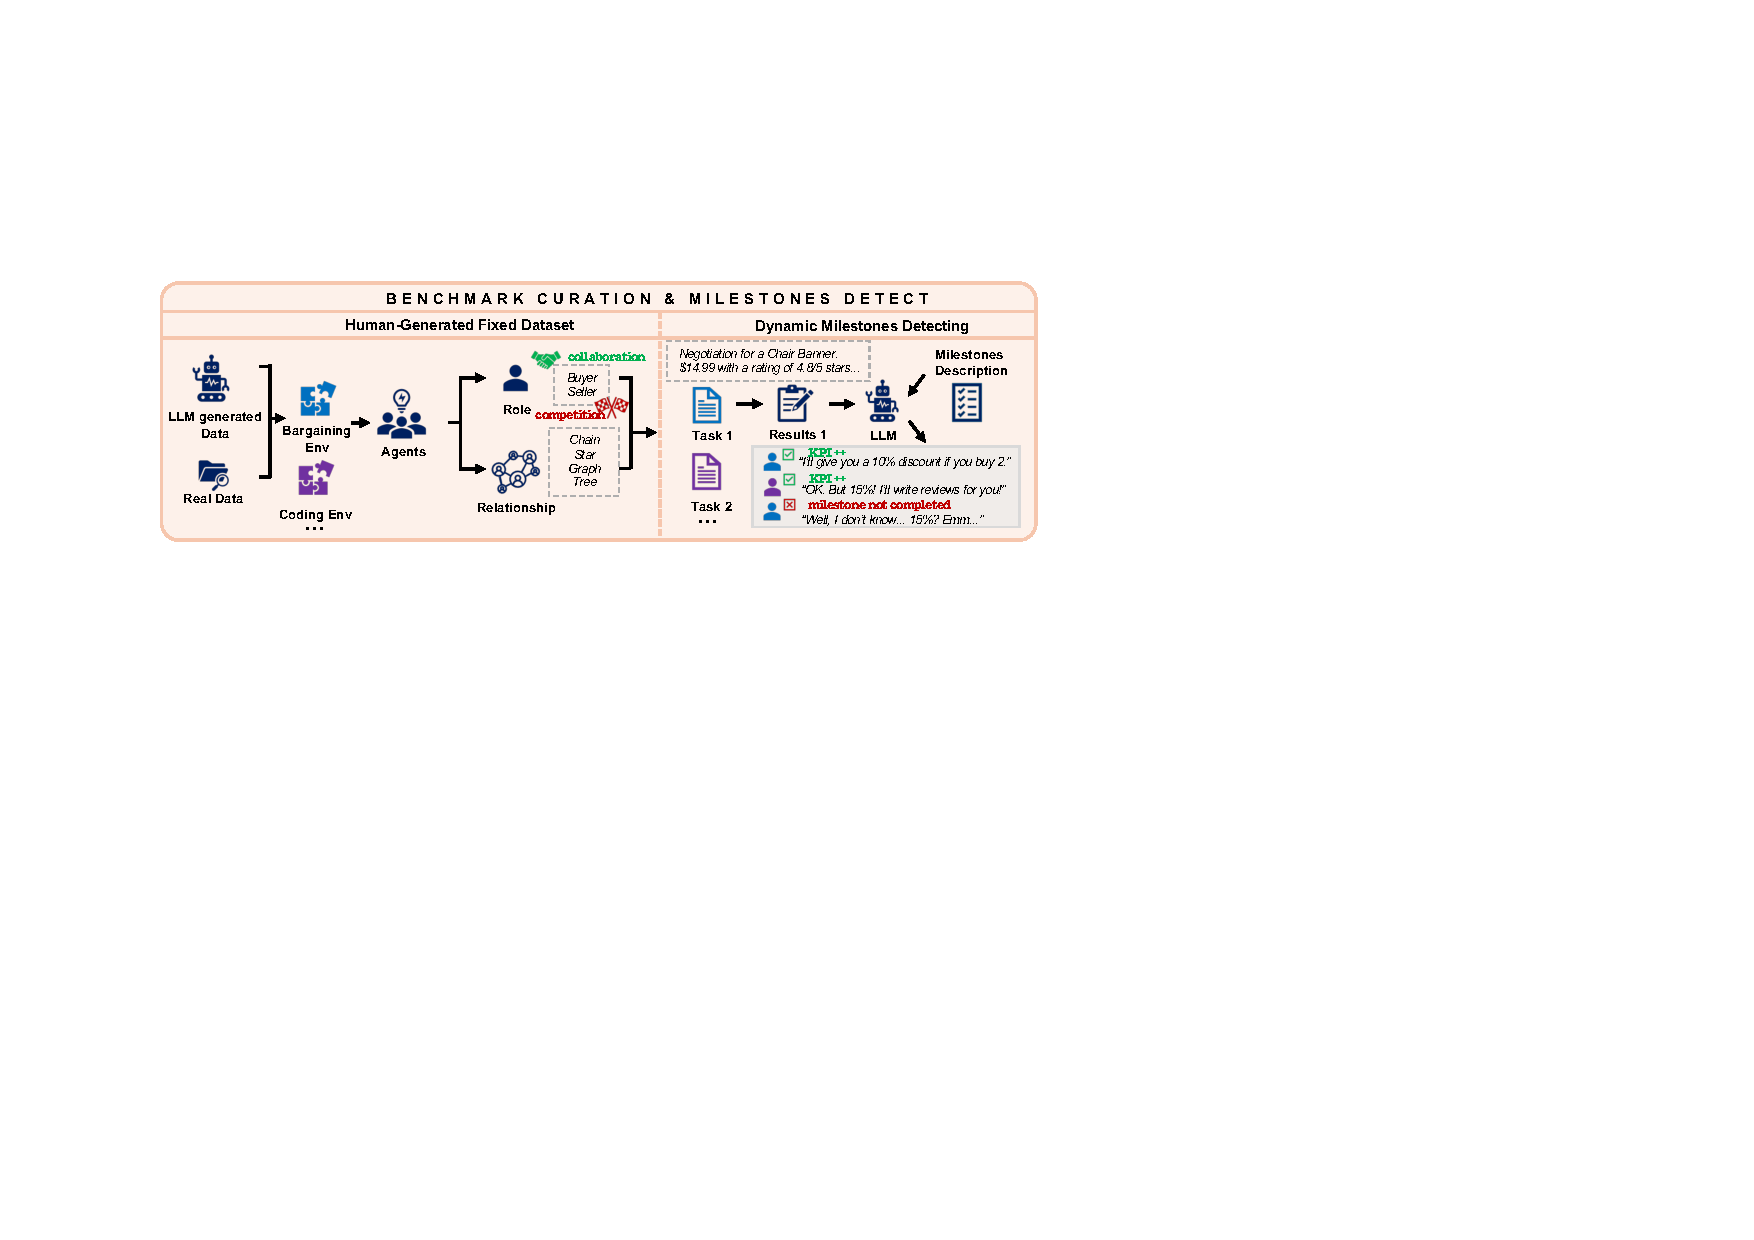
\includegraphics[width=\linewidth]{graphs/marble_graph.pdf}
%     \caption{Overview of the methodology: illustrating the milestones generation process, evaluation inputs for iterations, and metrics for task completion and coordination. Key components include task-based evaluation, KPI tracking, and collaboration between agents through planning, action, and communication.}
%     \label{fig:method}
% \end{figure*}
